\documentclass[border=10pt]{standalone}
\usepackage{tikz}
\usetikzlibrary{arrows.meta, calc}

\begin{document}
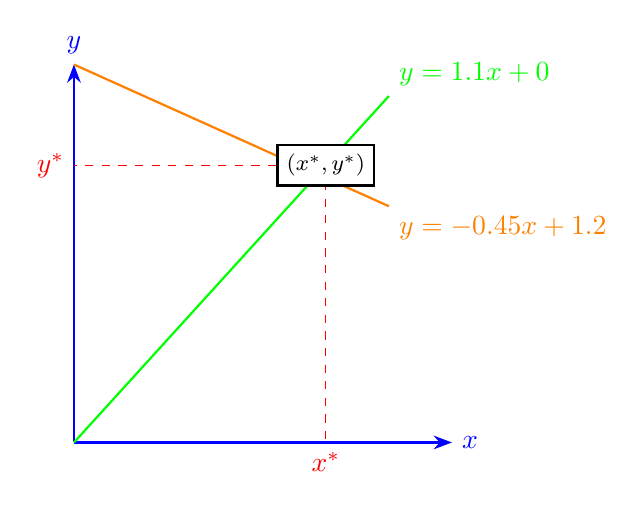
\begin{tikzpicture}[scale=4, >=Stealth]

% Axes
\draw[thick, blue, ->] (0,0) -- (1.2,0) node[right] {$x$};
\draw[thick, blue, ->] (0,0) -- (0,1.2) node[above] {$y$};

% Lines
\draw[thick, green] (0,0) -- (1.0, 1.1) node[above right] {$y = 1.1x + 0$};
\draw[thick, orange] (0,1.2) -- (1.0, 0.75) node[below right] {$y = -0.45x + 1.2$};

% Intersection point
\coordinate (P) at (0.8, 0.88);
\fill[blue] (P) circle (1.5pt);

% Dashed lines to axes
\draw[dashed, red] (P) -- (P |- 0,0) node[below] {$x^*$};
\draw[dashed, red] (P) -- (P -| 0,0) node[left] {$y^*$};

% Label for intersection point
\node[draw, thick, black, fill=white, align=center, font=\footnotesize] at (P) {$(x^*, y^*)$};

\end{tikzpicture}
\end{document}